\section{Gather your Witts}
To understand Borger's geometry over~${\mathbb{F}_{1}}$, rings of big Witt vectors are an indispensable tool. In this first post, some lesser known facts will be revealed about the man behind the ($p$-typical) ring, Ernst Witt.

\subsection{Nazi-Shmazi}
\begin{wrapfigure}[11]{r}{.35\textwidth}
  \centering
  \includegraphics[width=.3\textwidth]{playing-witt-rings/witt}
  \caption{Ernst Witt}
\end{wrapfigure}
How can it be that a ``typical, politically indifferent researcher'' joins the Nazi Party and wears his uniform to attend a seminar at a Jew's house? Witt's legacy is ridden with mysterious anecdotes and hearsay, all contributing to the opaque shroud surrounding the Witt ring. Surely, Witt's dominating features, honesty and straightforwardness, should be taken a lot more serious than they have been in the past.

\subsection{In God we trust}
Witt's grandfather was known to sacrifice everything for his faith, and expected the same from his family, which occupied a mild second place in his mind. To illustrate, you should check out his (kind of freaky) \href{http://www.norddeutsche-lehrer-gemeinschaft.de/heinrich-witt.html}{`fanpage'}, which seems to be thoroughly maintained by likeminded ones. If you're into German, try reading the little biography, and have a good laugh. Much the same story can be made for Ernst's father, who dedicated his life to the China Home Mission. The man was so devoted, that he even plaited his hair (!) and wore Chinese garments, so as to gain the confidence of the locals. Having a rather demanding job, he didn't spend at all much time with his children, who were educated strictly under the banner of honesty and religion. It is in this highly secular background that the stories surrounding Witt should be interpreted.

\subsection{Grounding live wires}
\begin{wrapfigure}{r}{.35\textwidth}
  \centering
  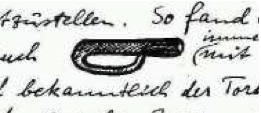
\includegraphics[width=.3\textwidth]{playing-witt-rings/klein}
  \caption{Ernst Witt}
\end{wrapfigure}
Even though Witt's work is mostly algebraic, one gets the impression he had a great intuition for studying problems, important to the whole of mathematics. Many of his highly original works have only shown their true power years after publishing. Witt also had a very broad knowledge of mathematics, physics, and a keen sense of visualization. To a large extent this seems to have been due to his favourite professors, Herglotz, Hasse, Artin and Noether. Witt had a tremendous respect for these people, as you can tell by looking at their long lasting correspondence. Behold part of a letter he sent to Herglotz in '43, highlighting some of his qualities (look at the picture!):
\begin{quote}
  \textsl{The time of mathematical expeditions is over for the time being, and I can just make some short walks in an already familiar mathematical territory. Occasionally, however, I succeed in finding an unknown plant there as well. So I realized that the Klein bottle can always be coloured with six colours, whereas the torus needs seven colours, as is well-known, although the topological `connectivity number' 3 is the same in both cases and only the possibility of orientation is responsible for the difference.}
\end{quote}
Go ahead, try proving this yourself. If you get tired, google 'Heawood conjecture'.


\subsection{Wittgol}
To indulge our `tech savvies', a last example of Ernst's visionary gaze. As early as~'59, Witt realized that computers would revolutionize all branches of mathematics. To put this into perspective, let me summarize the number crunchers of the day: thousands of vacuum tubes. For more than twenty years, Witt spent a lot of time programming, and it wasn't until '82, when his institute got a new computer, that he started losing interest. The programmes themselves were rather advanced and served, among others, the classification of Steiner systems. In the process, Witt adapted the language Algol to what his students named `Wittgol'.

In the words of Sanford Segal:
\begin{quote}
  \textsl{Ernst Witt seems to have actually suited a usual caricature of a mathematician --- both heedless and ignorant of the world, somewhat naive, self-absorbed in his mathematical universe, truly unpolitical. This is also a caricature sometimes used to explain academic reaction to the Nazis. In both cases it is almost always false. Witt is worth consideration because his life seems to show that the caricatures could, in fact, both be true.}
\end{quote}

If anyone wants to know more about the events I've been hinting at, check out the biography of Ernst Witt in~\cite{quadratic-forms}, \href{http://www.maths.ed.ac.uk/~aar/books/dublin.pdf}{freely available online}.

Next up, his work!
